\chapter{Release 2 : Consolidation groupe, catalogue standard et workflow budgétaire}
\label{chap:release2}


\section*{Introduction}

Ce quatrième chapitre présente la réalisation de la \textbf{Release 2}, combinant le \textbf{Sprint 3} (moteur de consolidation mondiale \textit{Cofat Group} et catalogue centralisé \textit{StandardInvestment}) et le \textbf{Sprint 4} (workflow du budget non-industriel, notifications temps réel et exportation de rapports).

\section{Sprint 3 : Module de consolidation groupe et catalogue des équipements standards}

\subsection{Objectifs du sprint 3}
Le Sprint 3 visait à offrir à la Direction Générale une vision consolidée en temps réel des capacités des 10 sites mondiaux et à centraliser le référentiel d'investissement \textit{StandardInvestment}.

\subsection{Backlog du sprint 3}
Le Tableau \ref{tab:backlog_sprint3} récapitule le backlog du Sprint 3 dédié à la consolidation mondiale et au catalogue Standard Investment.

\begin{table}[H]
\centering
\begin{tabular}{|c|p{9.2cm}|c|c|}
\hline
\textbf{Id} & \textbf{Fonctionnalités (User Story)} & \textbf{Priorité} & \textbf{Estimation (Jours)} \\ \hline
28 & En tant qu'Administrateur, je veux consolider en temps réel les besoins machines des 10 sites via des requêtes SQL \texttt{SUM} et \texttt{GROUP BY}. & 1 & 4 \\ \hline
29 & En tant qu'Administrateur, je veux consolider les parcs de machines disponibles pour obtenir la cartographie mondiale du groupe. & 1 & 3 \\ \hline
30 & En tant qu'Administrateur, je veux calculer le taux de charge moyen mondial par type d'équipement pour identifier les goulots d'étranglement. & 1 & 3 \\ \hline
31 & En tant qu'Administrateur, je veux identifier les opportunités de transfert d'équipements excédentaires entre usines du groupe. & 1 & 3 \\ \hline
32 & En tant qu'Administrateur, je veux consolider l'occupation spatiale de l'ensemble des usines afin de détecter les risques de saturation. & 1 & 3 \\ \hline
33 & En tant qu'Administrateur, je veux identifier les usines prioritaires pour des extensions de bâtiments industriels. & 2 & 2 \\ \hline
34 & En tant qu'Administrateur, je veux consolider les effectifs MOD et MOI mondiaux par site, par client et par catégorie de métier. & 1 & 3 \\ \hline
35 & En tant qu'Administrateur, je veux visualiser la courbe de montée en charge RH mondiale (Ramp-up) sur 36 mois. & 1 & 2 \\ \hline
36 & En tant qu'Acheteur, je veux consulter le catalogue centralisé des équipements standards (\textit{StandardInvestment}). & 1 & 2 \\ \hline
37 & En tant qu'Acheteur, je veux ajouter et paramétrer des équipements standards (cadence nominale, durée de vie, constructeur). & 1 & 2 \\ \hline
38 & En tant qu'Acheteur, je veux mettre à jour les coûts standards d'acquisition dans les devises internationales (EUR, BRL, MXN, USD). & 1 & 2 \\ \hline
39 & En tant qu'Acheteur, je veux rechercher et filtrer le catalogue standard par opération technique et type de machine. & 2 & 1 \\ \hline
\end{tabular}
\caption{Backlog du Sprint 3}
\label{tab:backlog_sprint3}
\end{table}

\subsection{Spécification des besoins fonctionnels}
Le moteur de consolidation agrège les données des 10 sites via des requêtes SQL \texttt{GROUP BY} avec \texttt{sequelize.fn('SUM')}.

\begin{figure}[H]
    \centering
    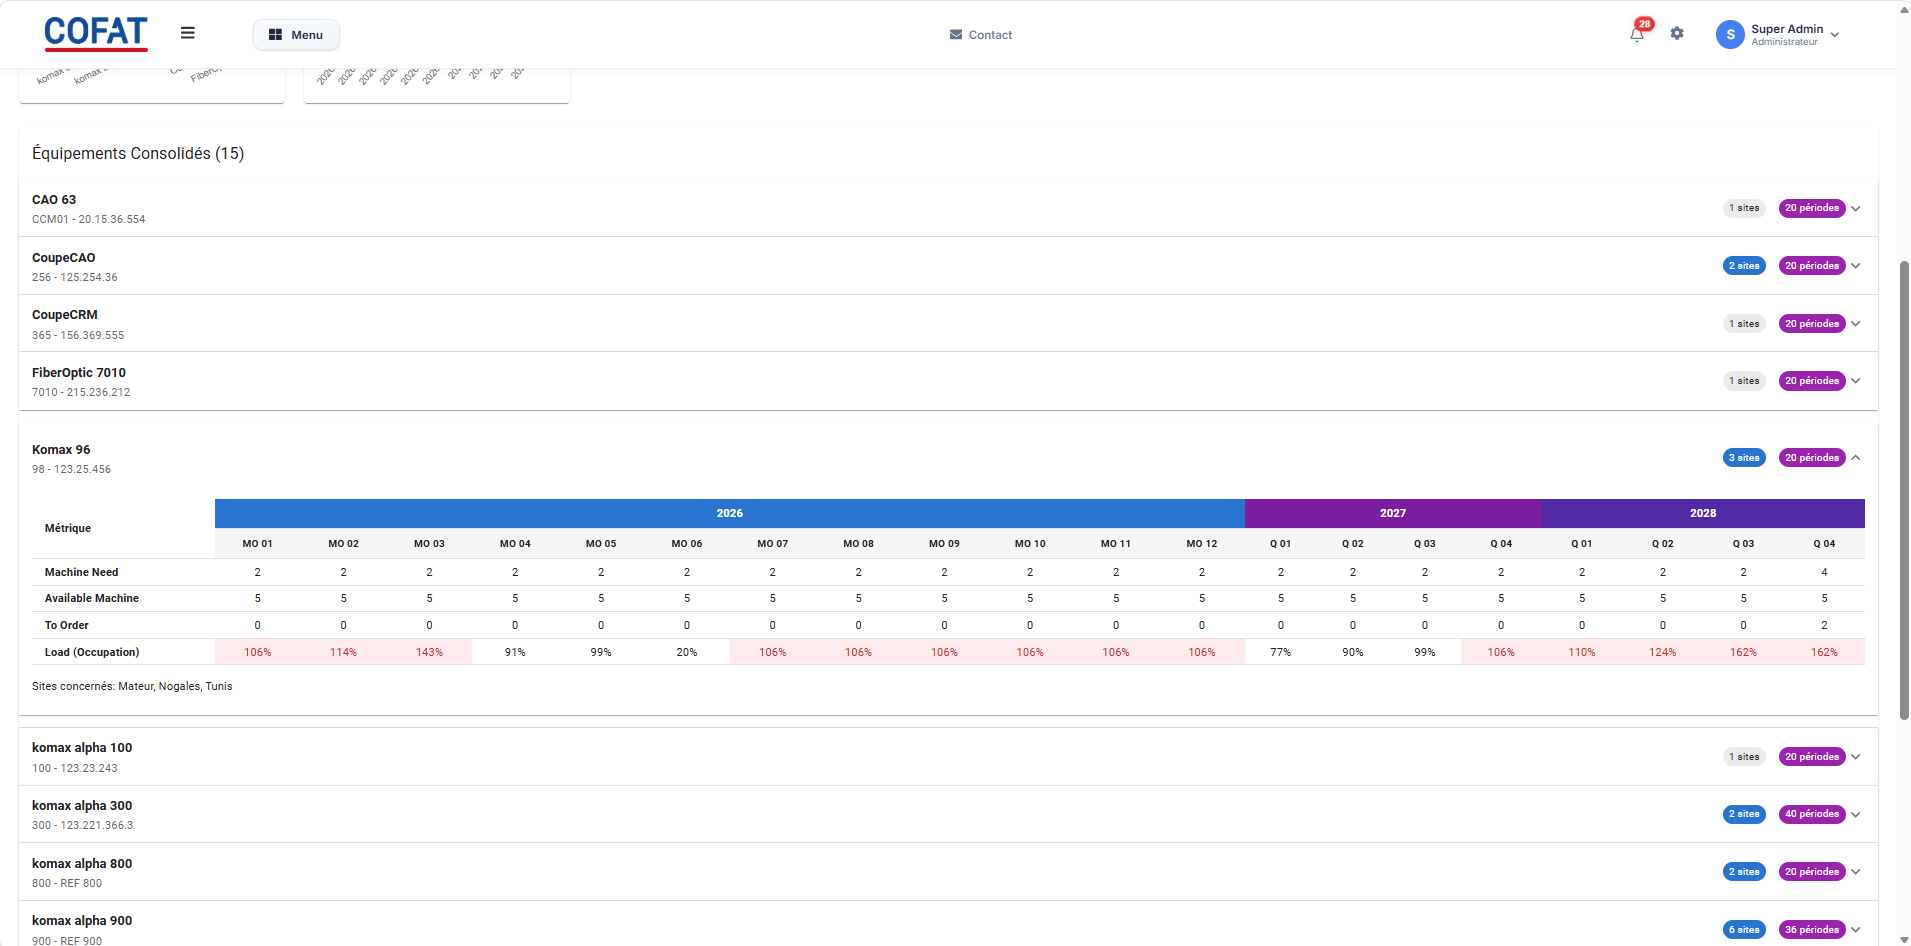
\includegraphics[width=0.9\textwidth]{img/consolidation_equipements.png}
    \caption{Tableau de consolidation mondiale des équipements industriels}
    \label{fig:conso_eq_ch4}
\end{figure}

\begin{figure}[H]
    \centering
    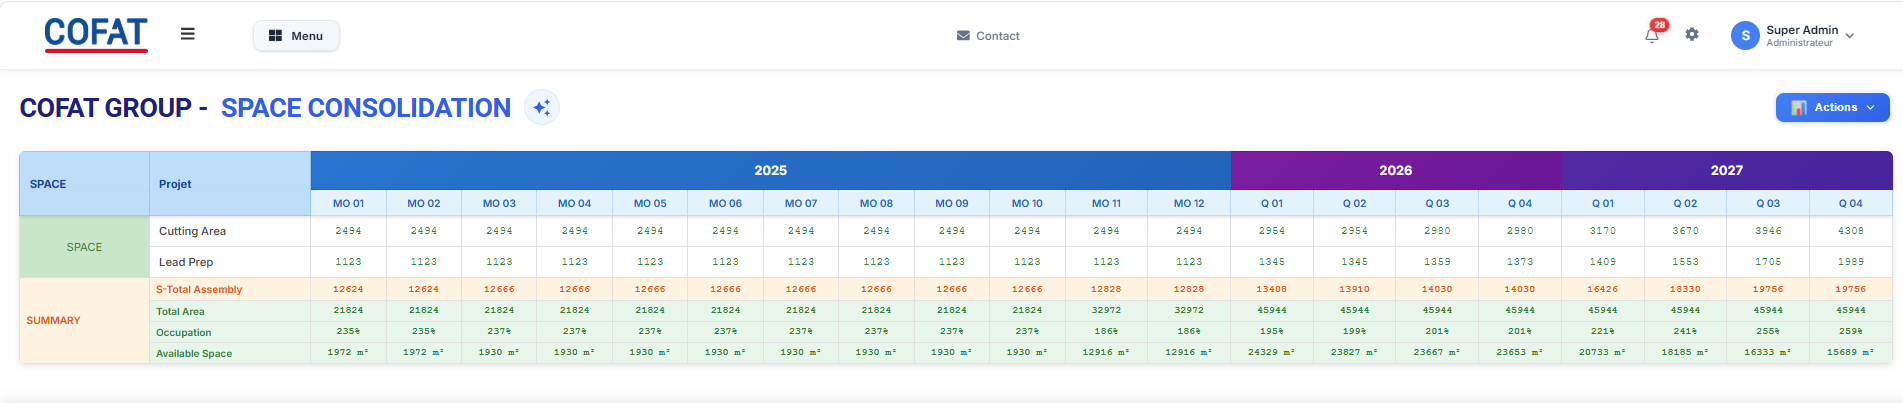
\includegraphics[width=0.9\textwidth]{img/consolidation_espaces.png}
    \caption{Consolidation mondiale de l'occupation des usines COFAT}
    \label{fig:conso_sp_ch4}
\end{figure}

\begin{figure}[H]
    \centering
    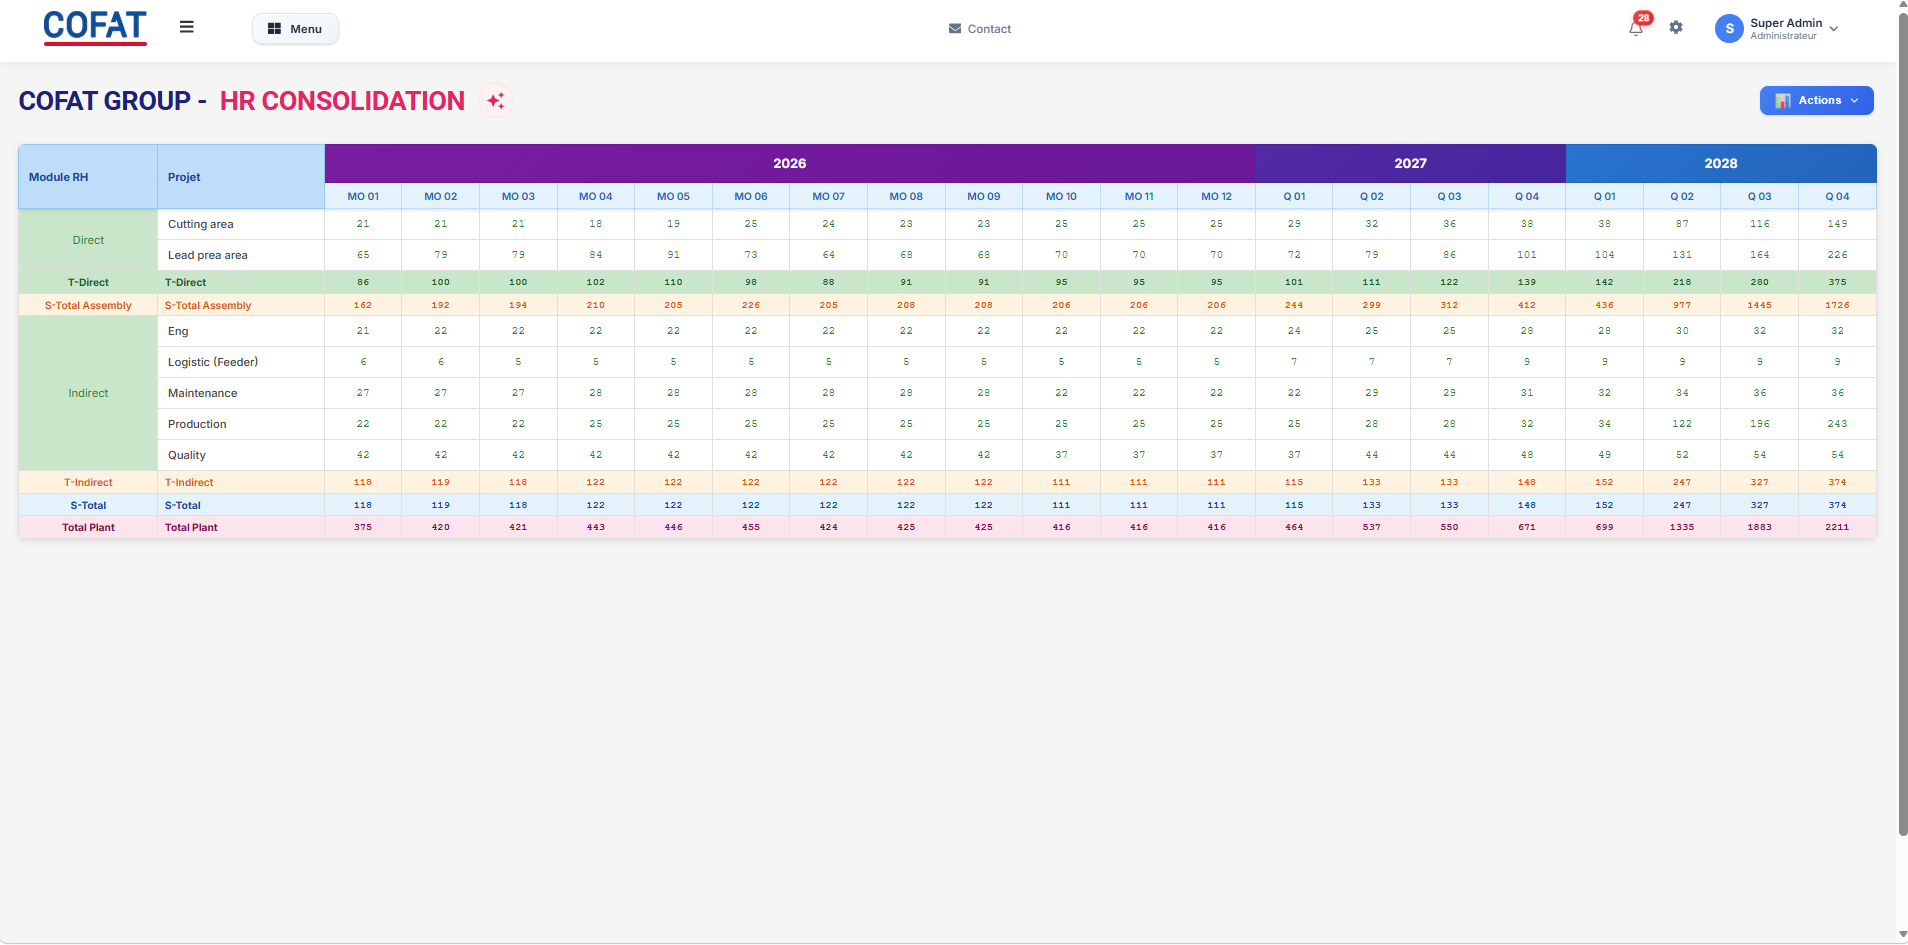
\includegraphics[width=0.9\textwidth]{img/consolidation_rh.png}
    \caption{Tableau de consolidation RH mondial par projet et catégorie}
    \label{fig:conso_hr_ch4}
\end{figure}

\begin{figure}[H]
    \centering
    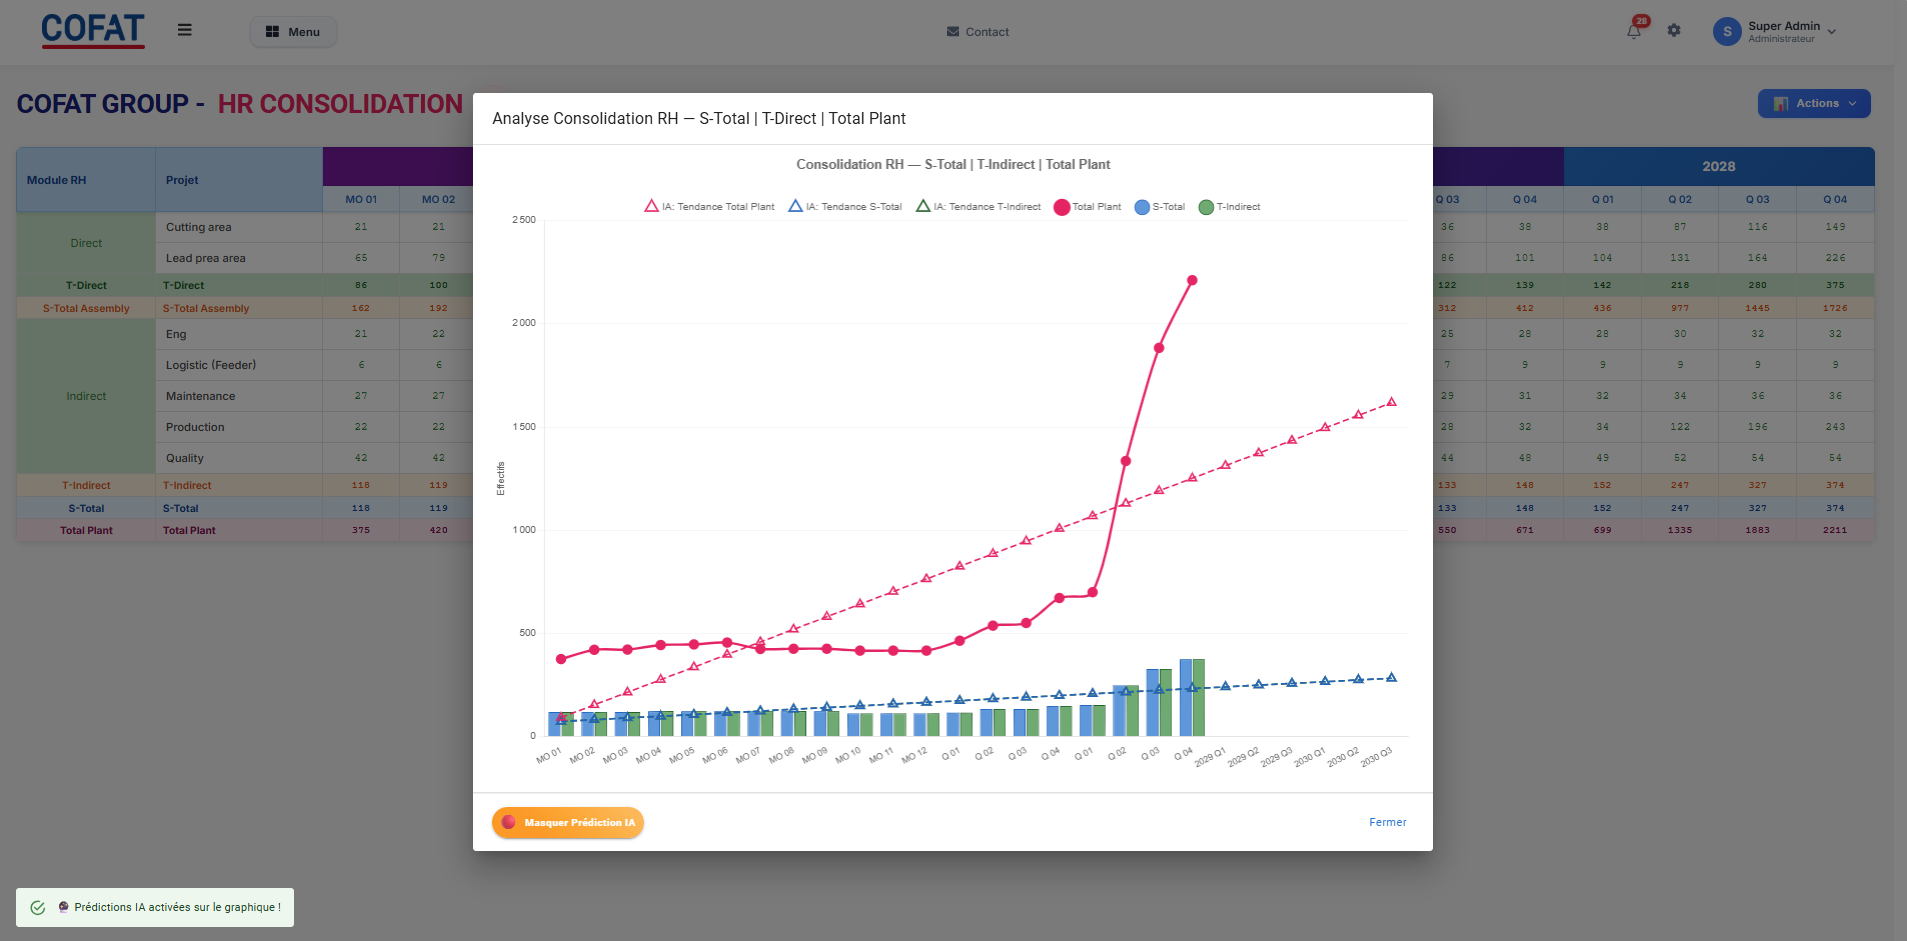
\includegraphics[width=0.85\textwidth]{img/dashboard_rh_rampup.png}
    \caption{Dashboard analytique de la montée en charge RH mondiale (Ramp-up)}
    \label{fig:dash_hr_ch4}
\end{figure}

Le catalogue \textit{StandardInvestment} permet de fixer les grilles tarifaires mondiales des machines.

\begin{figure}[H]
    \centering
    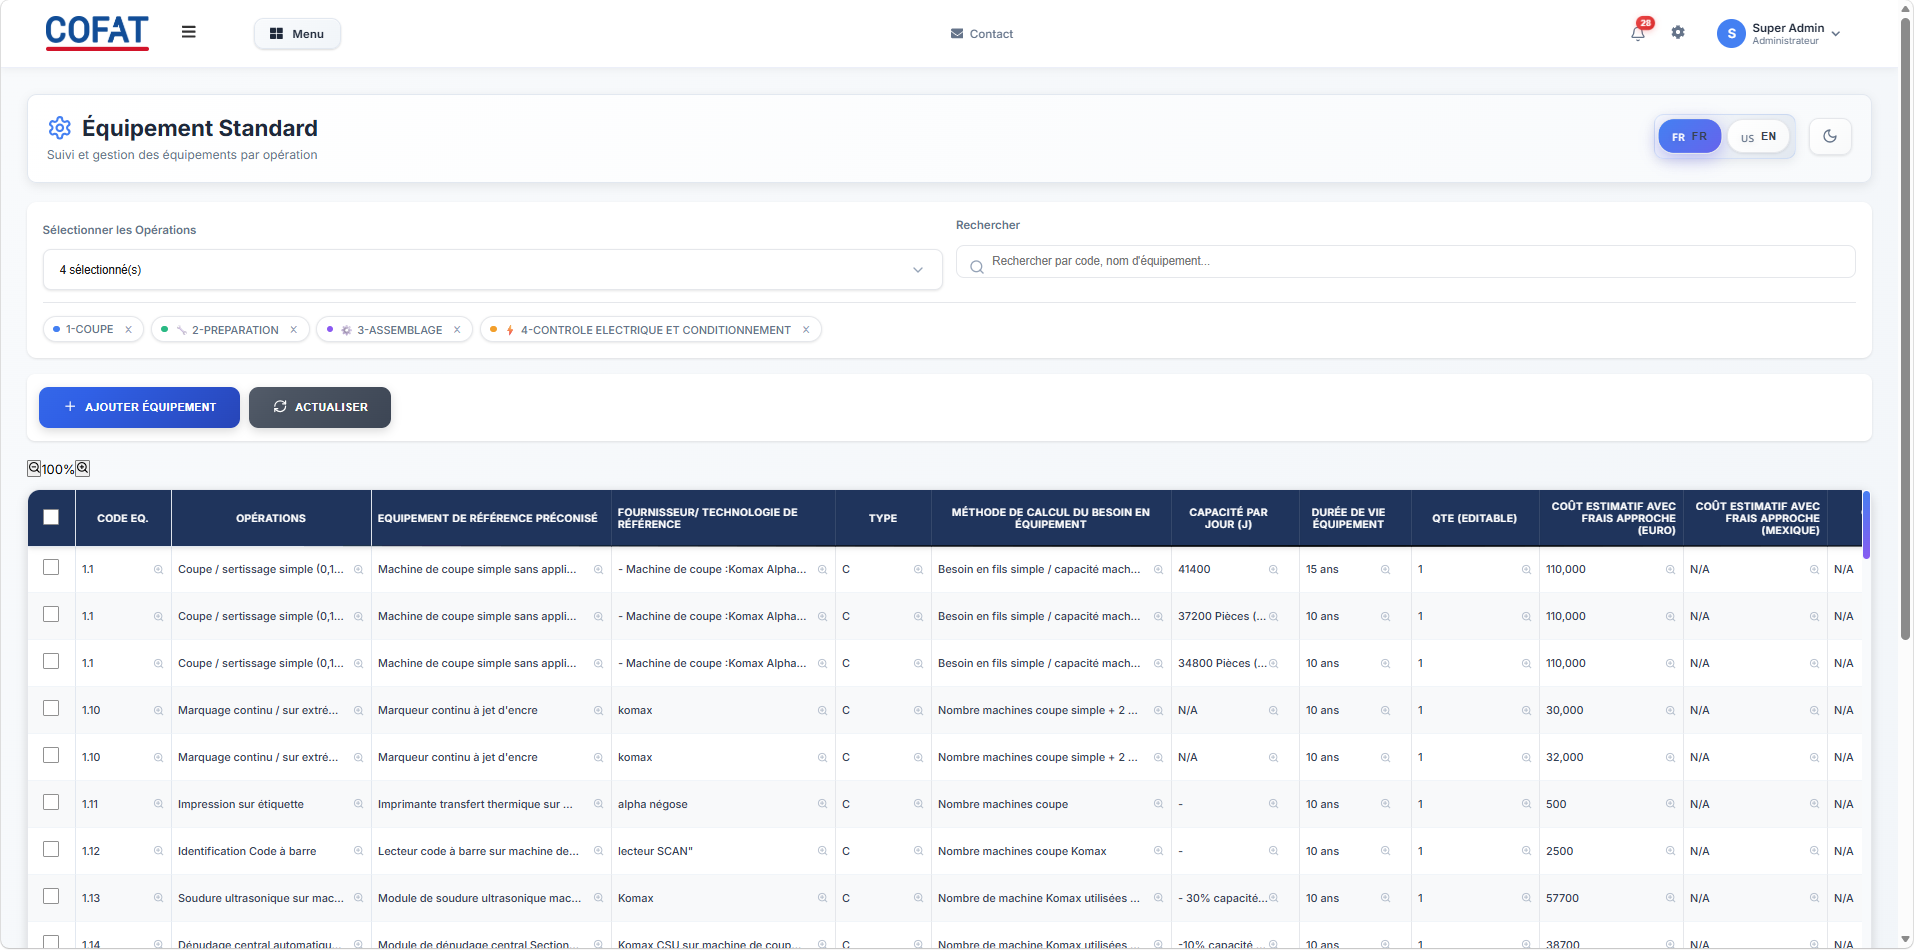
\includegraphics[width=0.9\textwidth]{img/catalogue_standardinvestment.png}
    \caption{Catalogue centralisé StandardInvestment}
    \label{fig:cat_std_ch4}
\end{figure}

\begin{figure}[H]
    \centering
    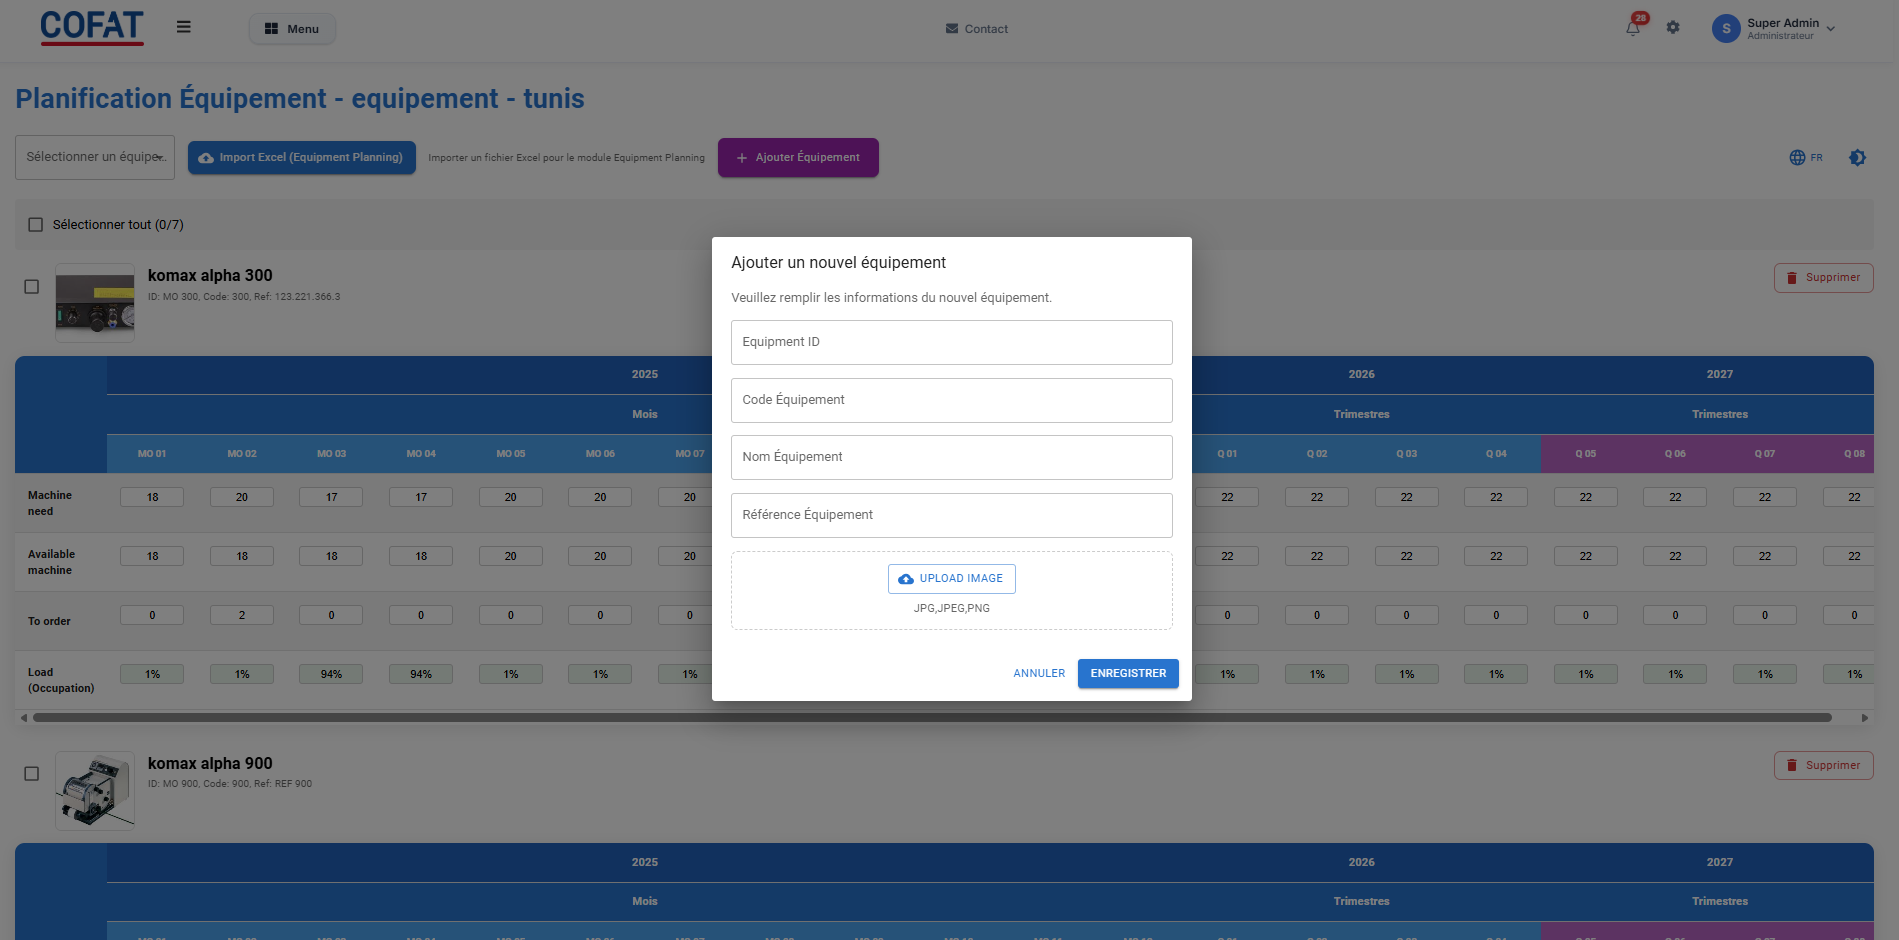
\includegraphics[width=0.85\textwidth]{img/form_std_part1.png}
    \caption{Formulaire d'ajout d'un équipement standard (Partie 1)}
    \label{fig:form_p1_ch4}
\end{figure}

\begin{figure}[H]
    \centering
    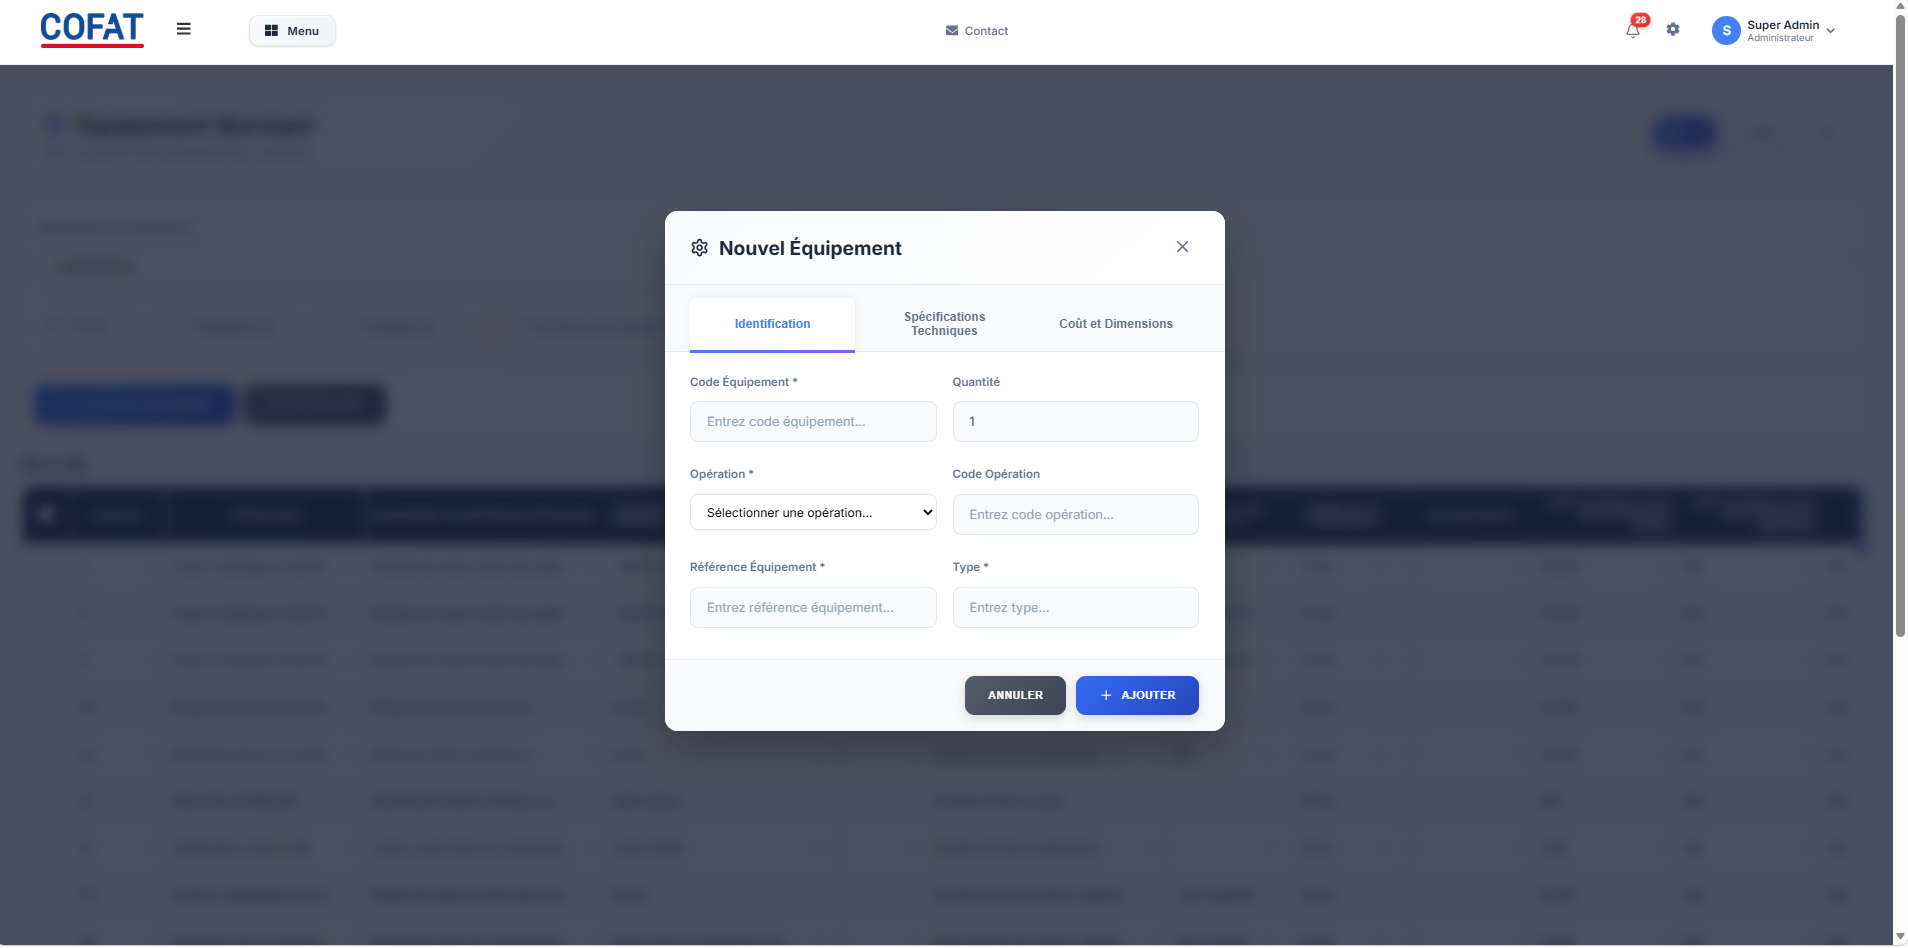
\includegraphics[width=0.85\textwidth]{img/form_std_part2.png}
    \caption{Formulaire d'ajout d'un équipement standard (Partie 2 : Coûts)}
    \label{fig:form_p2_ch4}
\end{figure}

\begin{figure}[H]
    \centering
    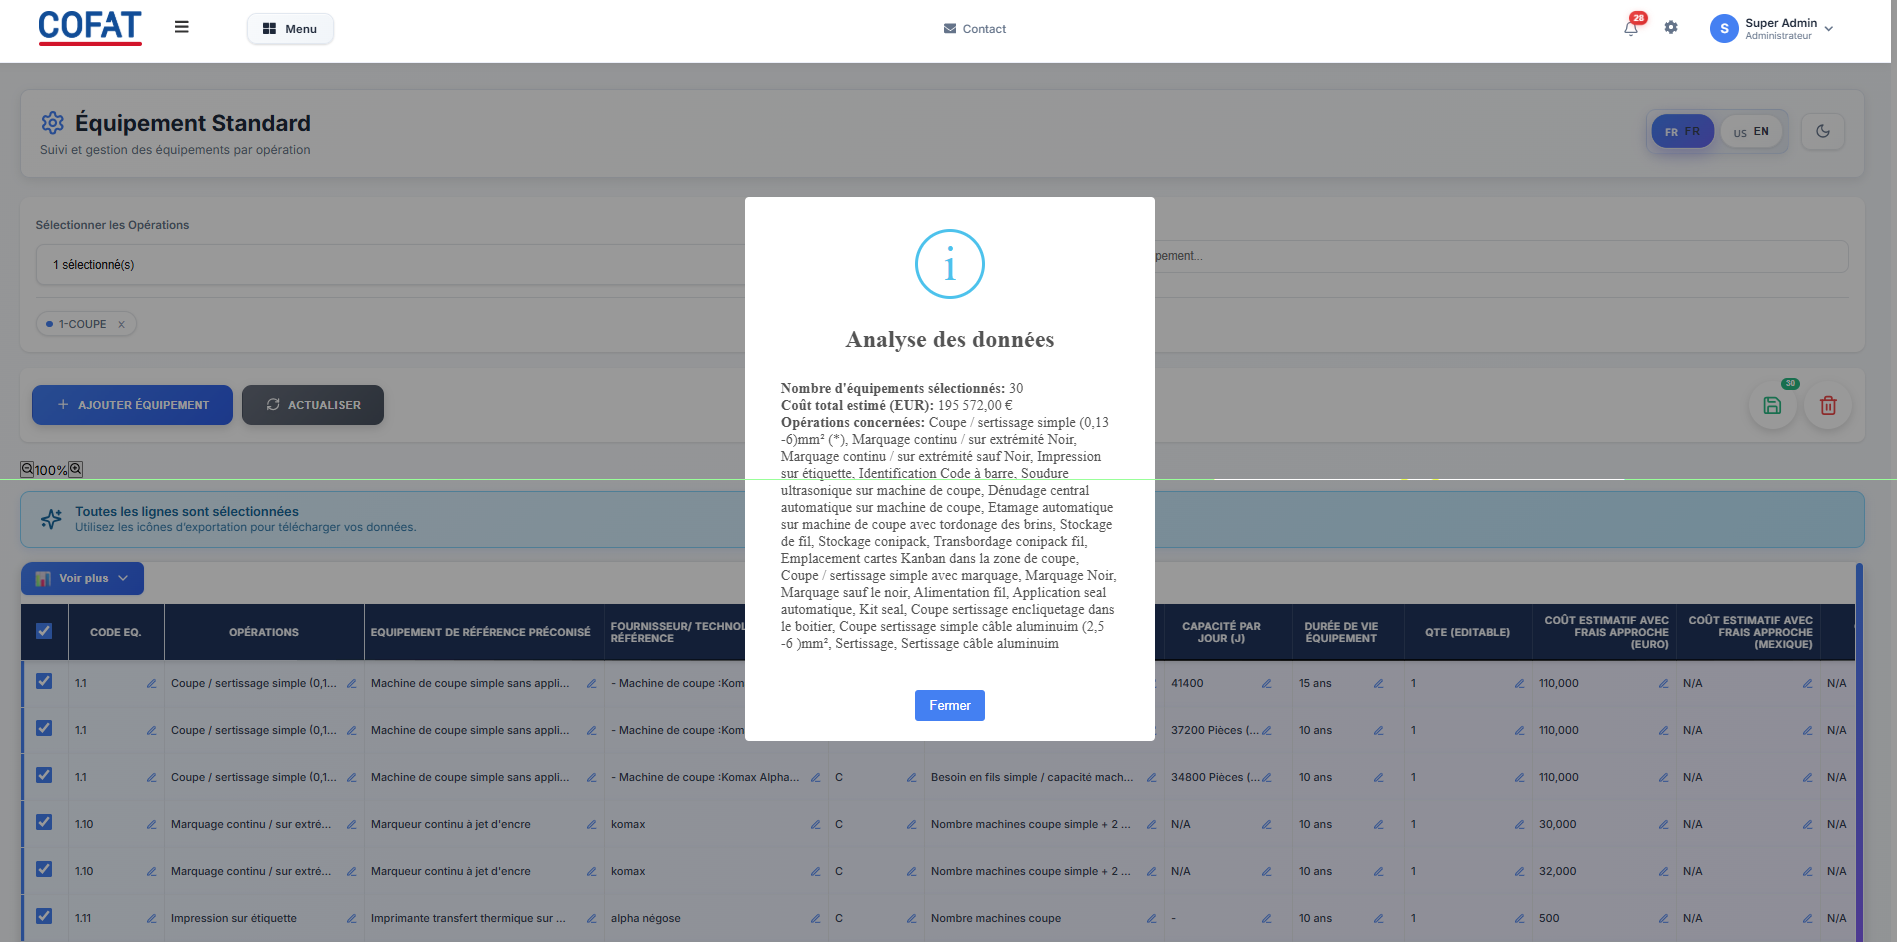
\includegraphics[width=0.85\textwidth]{img/analyse_stat_std.png}
    \caption{Fenêtre d'analyse des données du catalogue StandardInvestment}
    \label{fig:stat_std_ch4}
\end{figure}

\subsection{Diagramme de classes}
L'entité \texttt{StandardInvestment} gère les coûts régionaux (EUR, BRL, MXN).

\subsection{Diagrammes dynamiques}
L'agrégation des données de capacité est réalisée côté serveur via des requêtes Sequelize utilisant les fonctions SQL \texttt{SUM} et \texttt{GROUP BY} sur l'ensemble des 10 sites COFAT, garantissant une réponse en moins de 3 secondes.

\subsection{Réalisation}
Les tableaux de bord de consolidation permettent au Comité de Direction d'évaluer en temps réel la capacité globale du Groupe COFAT.

\subsubsection{Validation et recette du sprint 3}
Le Tableau \ref{tab:recette_r2_ch4} résume la recette fonctionnelle validée pour le Sprint 3.

\begin{table}[h]
\centering
\begin{tabular}{|p{1.5cm}|p{4.5cm}|p{5cm}|p{2.5cm}|}
\hline
\textbf{ID Test} & \textbf{Cas de test exécuté} & \textbf{Résultat attendu} & \textbf{Statut} \\ \hline
TEST-06 & Importation fichier Excel Équipements & Lecture .xlsx, calcul Load, bulkCreate BDD & \textbf{VALIDÉ} \\ \hline
TEST-07 & Importation fichier Excel invalide & Notification d'erreur avec ligne précise en échec & \textbf{VALIDÉ} \\ \hline
TEST-08 & Agrégation mondiale des 10 sites & Somme SQL temps réel des machines, réponse < 3s & \textbf{VALIDÉ} \\ \hline
TEST-09 & Modification prix StandardInvestment Achat & Seules les colonnes de prix sont modifiées & \textbf{VALIDÉ} \\ \hline
TEST-10 & Tentative modification libellé Achat & Requête rejetée par le contrôleur Express (HTTP 400) & \textbf{VALIDÉ} \\ \hline
\end{tabular}
\caption{Cahier de recette fonctionnelle du Sprint 3}
\label{tab:recette_r2_ch4}
\end{table}


\section{Sprint 4 : Module de gestion du budget non-industriel, notifications et exports}

\subsection{Objectifs du sprint 4}
Le Sprint 4 visait à numériser le workflow budgétaire entre les sites et le département Achats central, en restreignant strictement le rôle Achat à 2 colonnes (prix unitaire et devise) et en informant les utilisateurs via un système d'alertes instantanées.

\subsection{Backlog du sprint 4}
Le Tableau \ref{tab:backlog_sprint4} présente le backlog du Sprint 4 portant sur le workflow budgétaire non-industriel, les notifications et le reporting.

\begin{table}[H]
\centering
\begin{tabular}{|c|p{9.2cm}|c|c|}
\hline
\textbf{Id} & \textbf{Fonctionnalités (User Story)} & \textbf{Priorité} & \textbf{Estimation (Jours)} \\ \hline
40 & En tant que Site Manager, je veux créer une demande d'investissement non-industriel pour mon site de production. & 1 & 2 \\ \hline
41 & En tant que Site Manager, je veux affecter ma demande budgétaire à l'un des 7 départements industriels prédéfinis. & 1 & 1 \\ \hline
42 & En tant que Site Manager, je veux spécifier l'équipement requis, la quantité souhaitée, l'année d'achat et la justification. & 1 & 2 \\ \hline
43 & En tant que Site Manager, je veux soumettre formellement ma demande budgétaire au département Achats central. & 1 & 2 \\ \hline
44 & En tant qu'utilisateur, je veux qu'une notification système \texttt{NEW\_REQUEST} soit générée automatiquement lors de la soumission. & 1 & 3 \\ \hline
45 & En tant qu'Acheteur, je veux consulter la liste consolidée de toutes les demandes budgétaires non-industrielles des 10 sites. & 1 & 3 \\ \hline
46 & En tant qu'Acheteur, je veux filtrer et trier les demandes d'achat par site d'origine, par département et par état d'avancement. & 2 & 2 \\ \hline
47 & En tant qu'Acheteur, je veux modifier exclusivement les deux champs autorisés : le prix unitaire (\texttt{unitPrice}) et la devise (\texttt{currency}). & 1 & 3 \\ \hline
48 & En tant qu'Acheteur, je veux que toutes les autres colonnes de la demande soient strictement verrouillées en lecture seule. & 1 & 2 \\ \hline
49 & En tant qu'utilisateur, je veux que le serveur Sequelize recalcule instantanément le montant total (\texttt{totalPrice} = \texttt{qty} $\times$ \texttt{unitPrice}). & 1 & 2 \\ \hline
50 & En tant qu'Acheteur, je veux valider et enregistrer le chiffrage unitaire et la devise pour actualiser le montant total budgétaire. & 1 & 2 \\ \hline
51 & En tant que Site Manager, je veux recevoir une notification système \texttt{PRICE\_UPDATED} dès que l'Acheteur chiffre ma demande. & 1 & 2 \\ \hline
52 & En tant qu'utilisateur, je veux disposer d'un volet de notifications temps réel avec compteur de badges et marquage comme lu. & 2 & 3 \\ \hline
53 & En tant qu'utilisateur, je veux exporter les données consolidées de capacité et de budget au format tableur Excel (.xlsx). & 1 & 2 \\ \hline
54 & En tant qu'utilisateur, je veux générer et télécharger des rapports de synthèse budgétaire au format PDF imprimable. & 2 & 2 \\ \hline
55 & En tant qu'Administrateur, je veux visualiser les indicateurs graphiques de répartition des investissements par département et par usine. & 2 & 2 \\ \hline
\end{tabular}
\caption{Backlog du Sprint 4}
\label{tab:backlog_sprint4}
\end{table}

\subsection{Spécification des besoins fonctionnels}
Le workflow budgétaire se déroule de manière directe et fluide, sans étape d'approbation hiérarchique lourde :
\begin{enumerate}
    \item \textbf{Création du besoin :} Le Site Manager crée une ligne de budget d'investissement en renseignant le département cible (parmi les 7 départements industriels disponibles), l'équipement, la quantité et une estimation initiale. L'enregistrement déclenche immédiatement la notification système \texttt{NEW\_REQUEST} adressée au rôle Achat.
    \item \textbf{Tarification exclusive par l'Achat :} L'Acheteur consulte les lignes budgétaires créées et met à jour strictement les deux seules colonnes autorisées : le prix unitaire (\texttt{unitPrice}) et la devise (\texttt{currency}). Le serveur Sequelize calcule automatiquement le montant total (\texttt{totalPrice} = \texttt{qty} $\times$ \texttt{unitPrice}) et génère une notification \texttt{PRICE\_UPDATED} en retour vers le Site Manager.
\end{enumerate}

\begin{figure}[H]
    \centering
    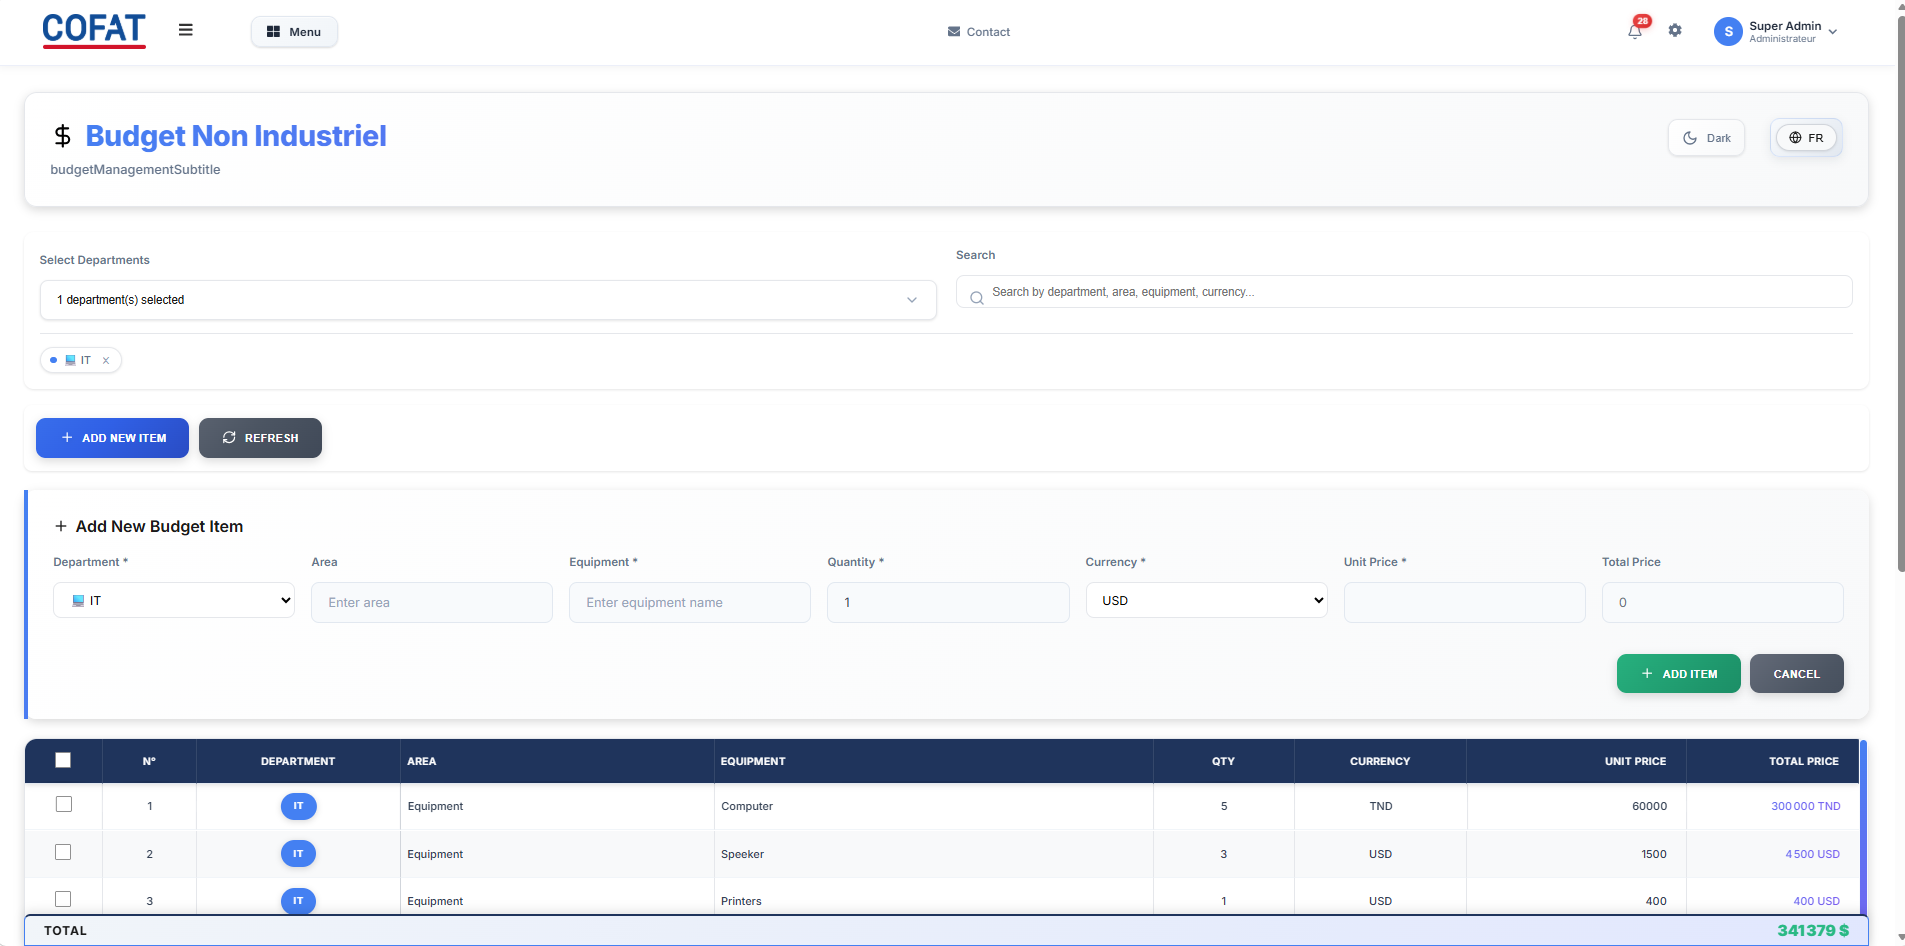
\includegraphics[width=0.9\textwidth]{img/budget_non_industriel.png}
    \caption{Interface de gestion dynamique du budget non-industriel}
    \label{fig:budget_ui_ch4}
\end{figure}

\begin{figure}[H]
    \centering
    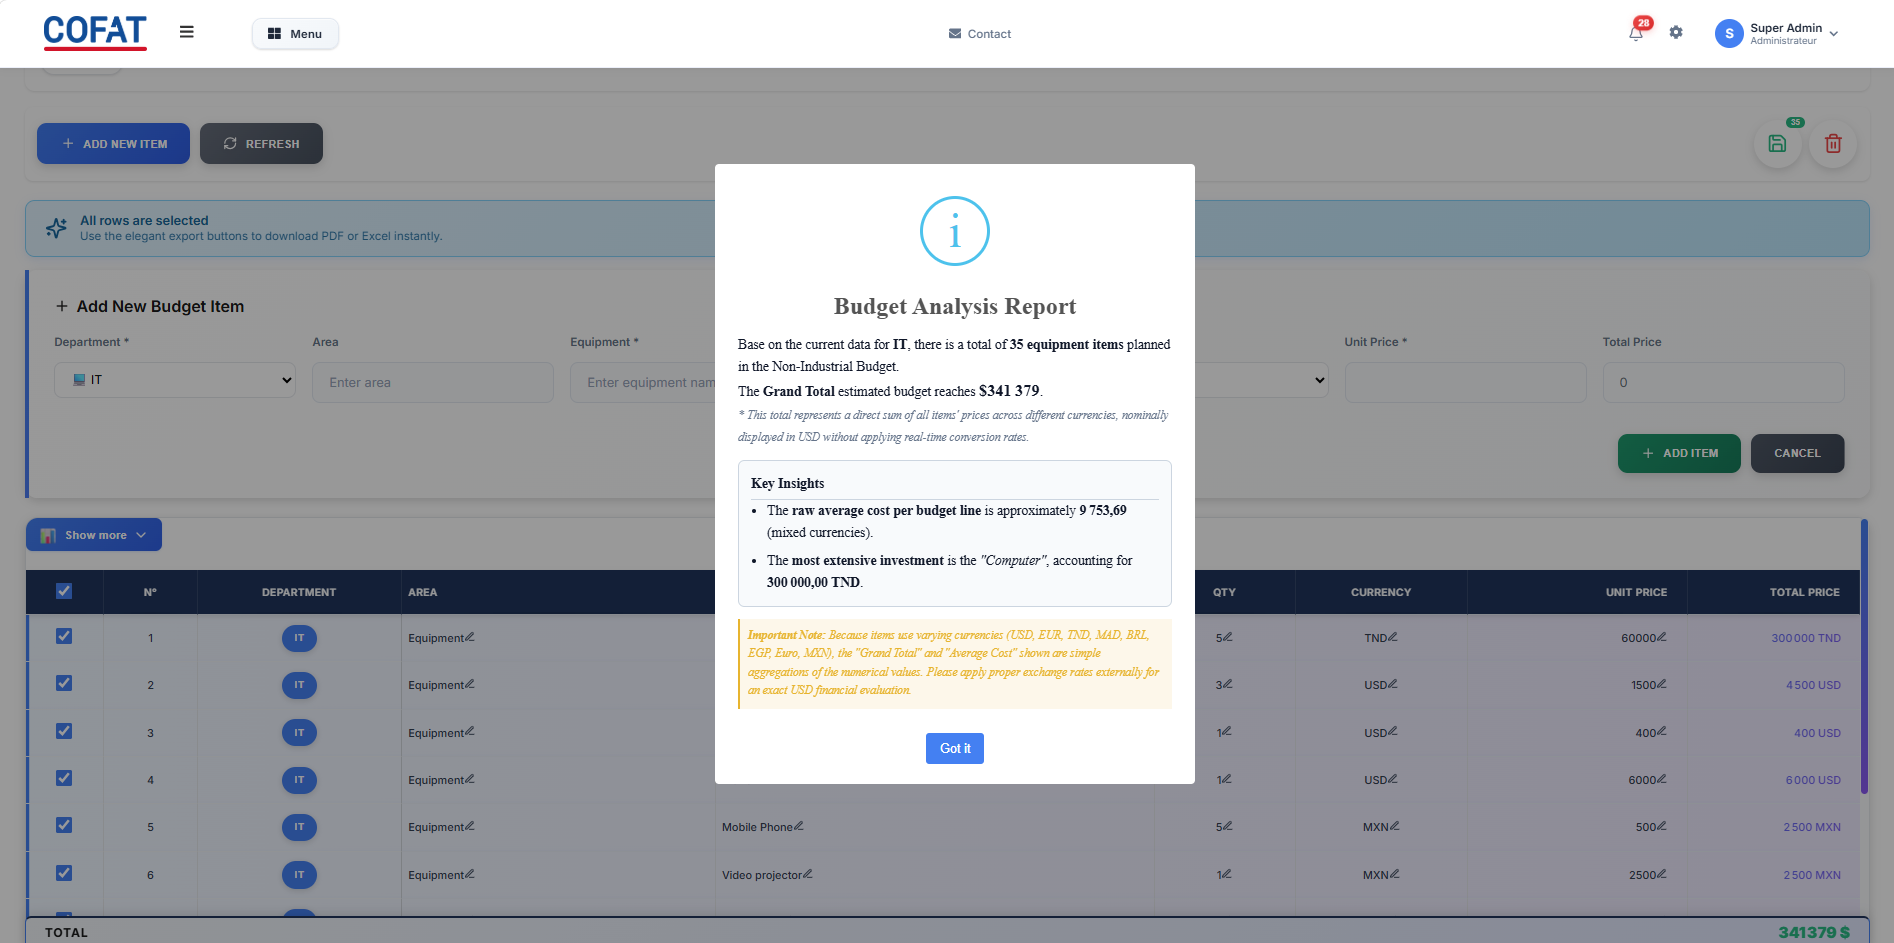
\includegraphics[width=0.9\textwidth]{img/dashboard_budget.png}
    \caption{Tableau de bord d'analyse des dépenses par département}
    \label{fig:budget_dash_ch4}
\end{figure}

\subsection{Diagramme de classes}
Les entités du Sprint 4 sont \texttt{NonIndustrialBudget} et \texttt{BudgetNotification}.

\subsection{Diagrammes dynamiques}
Le diagramme de séquence de la Figure \ref{fig:seq_budget_ch4} illustre le workflow de modification tarifaire et la notification automatique.

\begin{figure}[H]
    \centering
    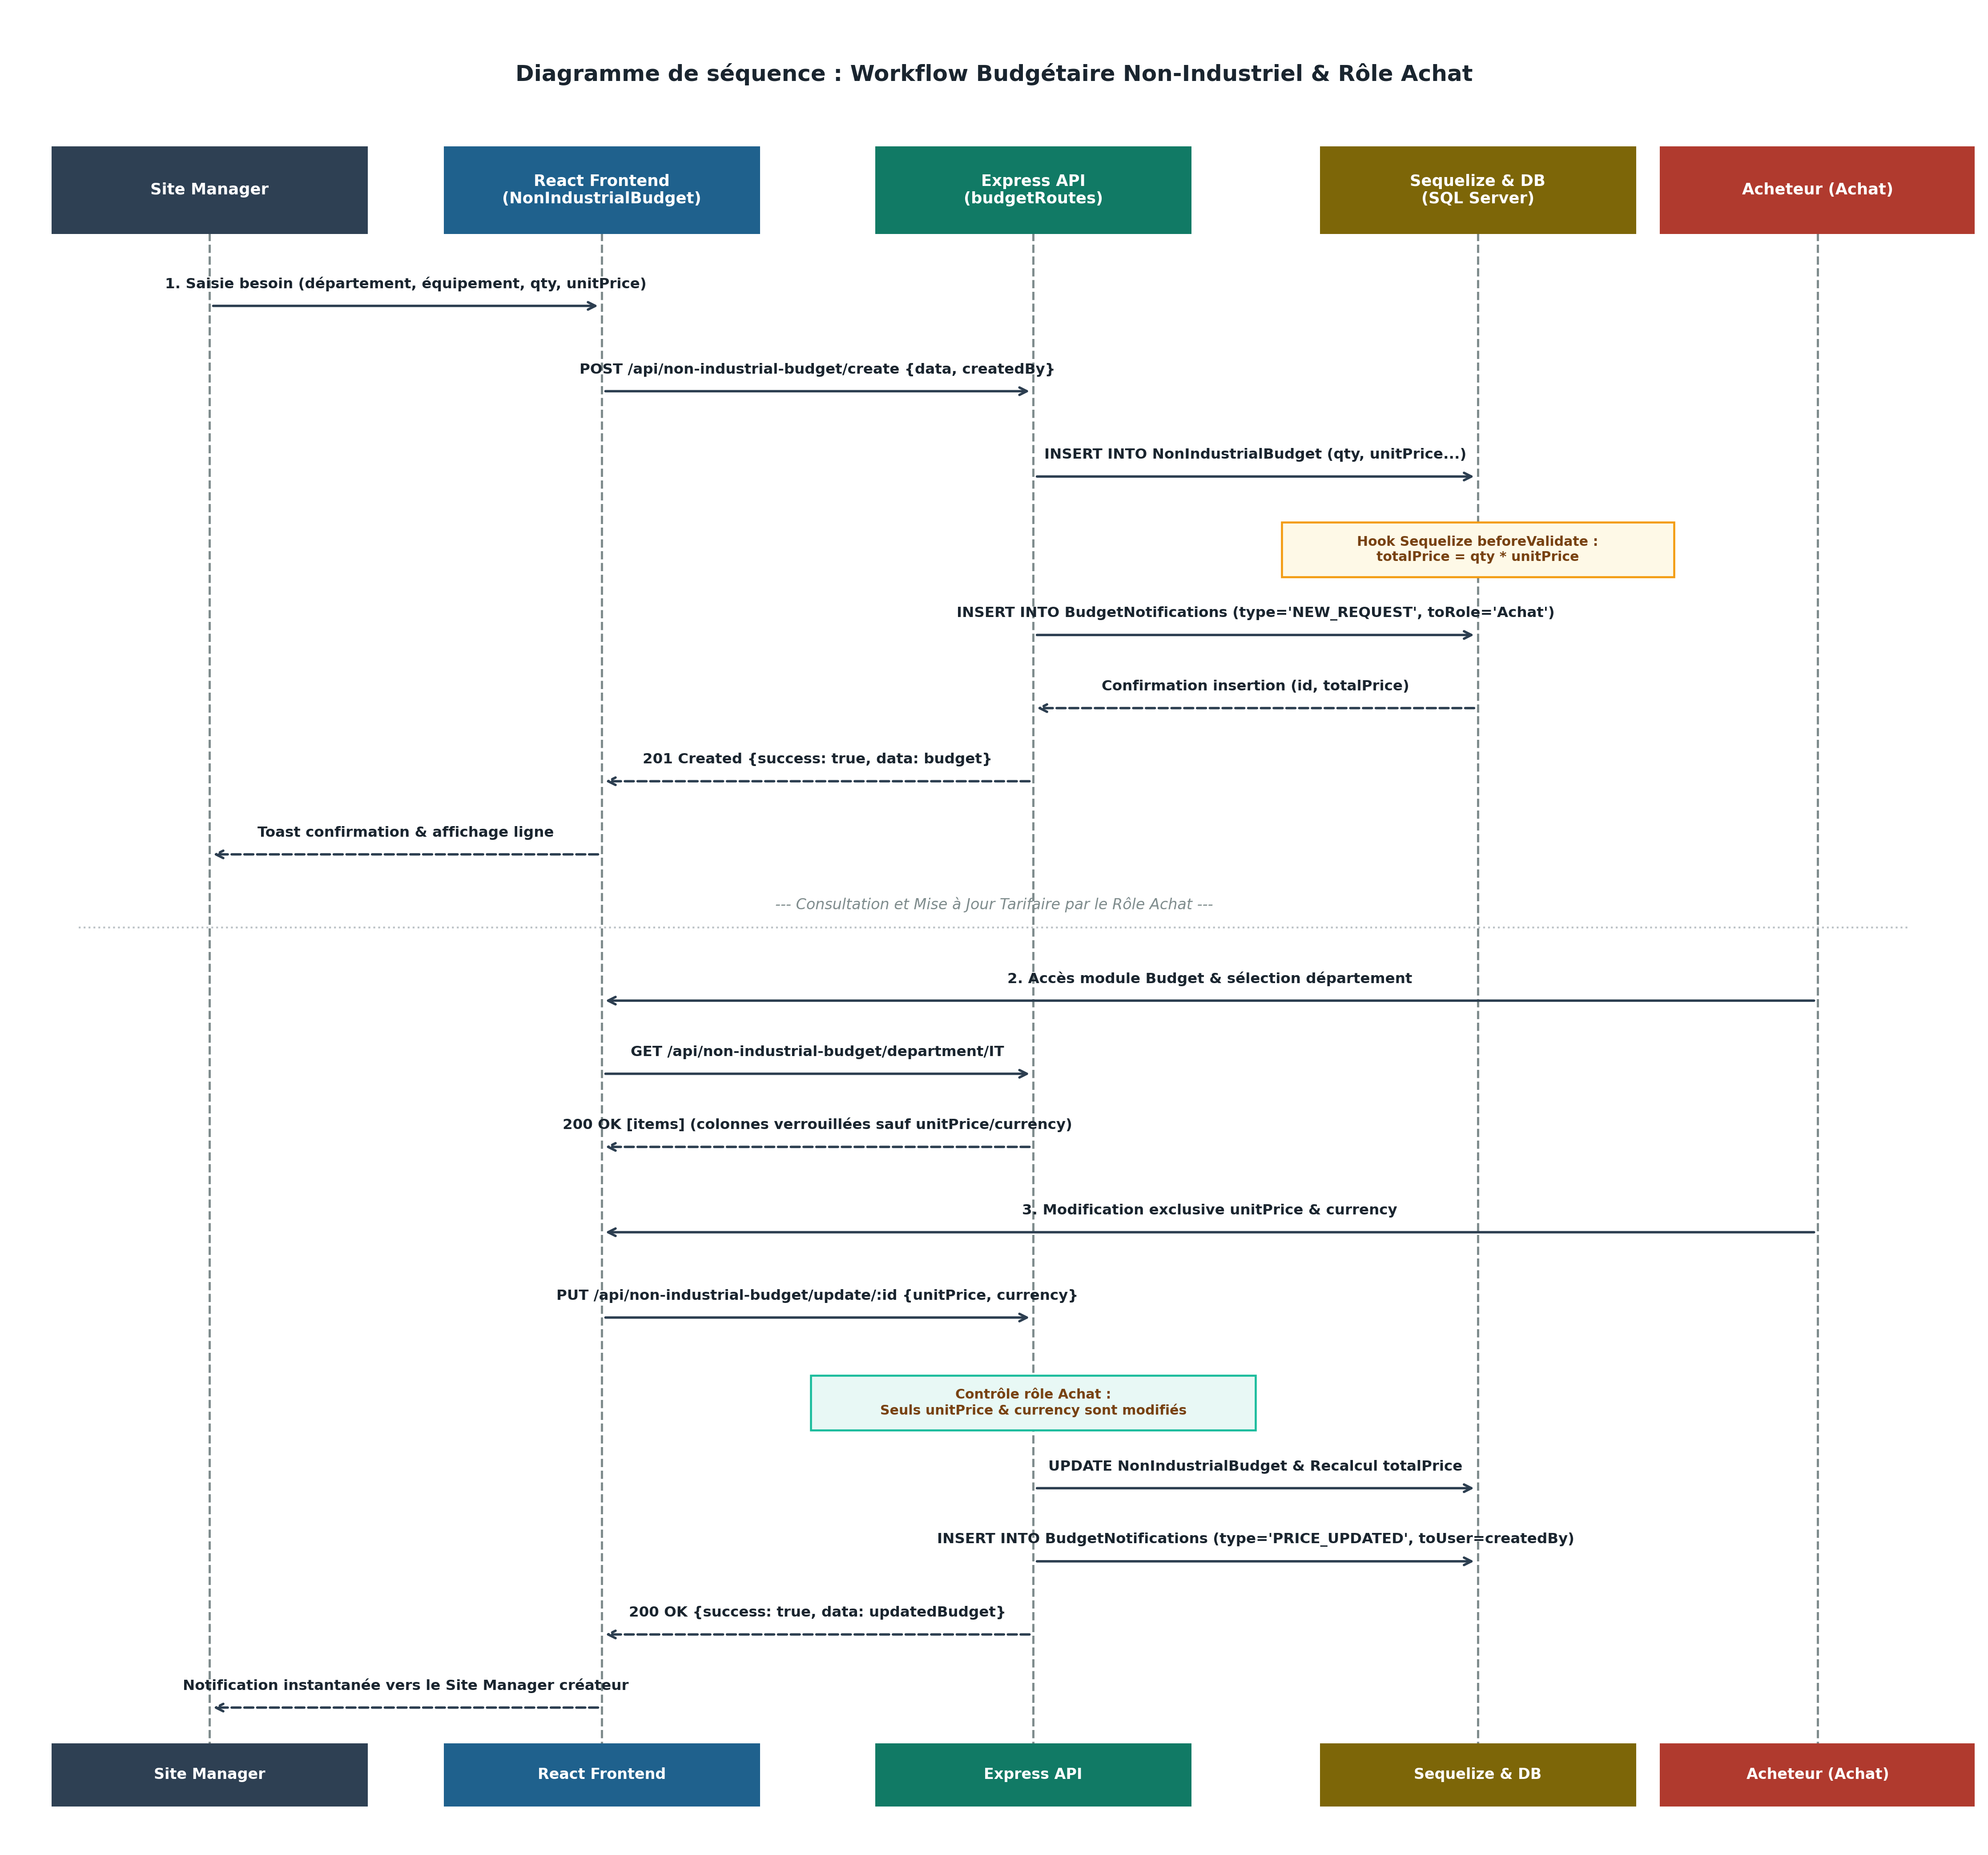
\includegraphics[width=0.85\textwidth]{img/sequence_workflow_achat.png}
    \caption{Diagramme de séquence du workflow de modification du prix par l'Achat}
    \label{fig:seq_budget_ch4}
\end{figure}


\subsection{Réalisation}
L'interface React adapte dynamiquement les champs éditables en fonction du rôle connecté (Achat vs Site Manager).

\subsubsection{Validation et recette du sprint 4}
Le Tableau \ref{tab:recette_s4_ch4} présente le cahier de recette validé pour le Sprint 4.

\begin{table}[h]
\centering
\begin{tabular}{|p{1.5cm}|p{4.5cm}|p{5cm}|p{2.5cm}|}
\hline
\textbf{ID Test} & \textbf{Cas de test exécuté} & \textbf{Résultat attendu} & \textbf{Statut} \\ \hline
TEST-11 & Soumission budget par Site Manager & Création ligne statut 'SUBMITTED', notification Achat & \textbf{VALIDÉ} \\ \hline
TEST-12 & Saisie prix unitaire par Acheteur & Mise à jour `unitPrice`, recalcul serveur de `totalPrice` & \textbf{VALIDÉ} \\ \hline
TEST-13 & Modification quantité par Achat & Action rejetée par le serveur, champ `qty` inchangé & \textbf{VALIDÉ} \\ \hline
TEST-14 & Polling notification cloche React & Incrémentation du compteur sans rechargement & \textbf{VALIDÉ} \\ \hline
TEST-15 & Exportation rapport Budget Excel & Téléchargement du fichier .xlsx avec en-têtes COFAT & \textbf{VALIDÉ} \\ \hline
\end{tabular}
\caption{Cahier de recette fonctionnelle du Sprint 4}
\label{tab:recette_s4_ch4}
\end{table}

\section*{Conclusion}
La Release 2 (Sprints 3 et 4) clôture l'ensemble des développements de la plateforme \textit{Cofat Capacity Study}.
